\documentclass[9pt]{article}
\usepackage{amsmath,amsfonts,times}
\usepackage{graphicx,color,tikz,pgfplots}
\usepackage[zswash]{mtpro2}
\usepackage[paperwidth=10cm,paperheight=10cm,lmargin=0in,rmargin=0in,tmargin=0.in,bmargin=0.in]{geometry}
\usepackage{bm}
\usetikzlibrary{arrows,shadings,shapes.arrows,decorations.pathreplacing,calc}
\usepgfplotslibrary{fillbetween}


\pagestyle{empty}
\pgfplotsset{compat=newest}
\definecolor{applered}{RGB}{255,8,0}
\definecolor{azure}{RGB}{0,127,255}
\definecolor{violet}{RGB}{159,0,255}

\pgfdeclareverticalshading{rainbow}{100bp}
{color(0bp)=(applered); color(25bp)=(red); color(40bp)=(yellow);
  color(47bp)=(green); color(51bp)=(cyan); color(60bp)=(blue);
  color(65bp)=(violet); color(100bp)=(violet)} 
                          
\newlength{\h}
\newlength{\rad}
\setlength{\h}{1.5cm}
\setlength{\rad}{.75pt}

\begin{document}
\centering
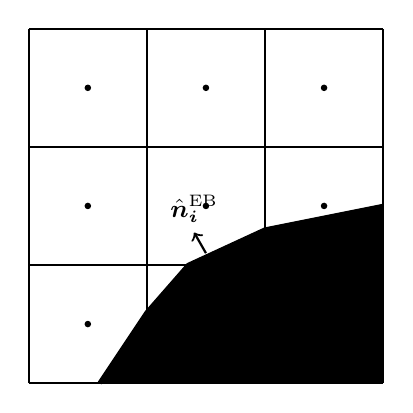
\begin{tikzpicture}[
    gridstyle/.style={thick,black},
    nodeCenterStyle/.style={thick,black,fill},
    nodeFaceStyle/.style={thick,black},
    VoFStyle/.style={font=\small,anchor = north west},
    surfaceStyle/.style={ultra thick,black},
    volumeStyle/.style={thick,densely dashed,black},
    surfaceFill/.style={},
    braceStyle/.style={thick,decorate,decoration={brace,amplitude=4pt,raise=2pt}},
    alphaStyle/.style={font=\small,anchor=east,xshift=-4pt},
    hTopStyle/.style={font=\small,anchor=east,yshift=4pt},
    hLeftStyle/.style={font=\small,anchor=east,xshift=-4pt},
    betaStyle/.style={font=\small,anchor=west,xshift=4pt},
    EBStyle/.style={font=\small,anchor=south,yshift=4pt},
    kappaStyle/.style={font=\small,anchor=center},
    normalStyle/.style={font=\small,->,thick,black},
    gradientStyle/.style={font=\small,->,thick,black},
    surfaceCharge/.style={font=\small,yshift=2pt},
    phiStyle/.style={font=\small,anchor=south},
  ]

  %% Grids and nodes
  \draw[step=\h,gridstyle] (0,0) grid (3\h,3\h);
  \foreach \x in {\h/2,3\h/2,5\h/2} {
    \foreach \y in {\h/2,3\h/2,5\h/2} {
      \draw[nodeCenterStyle] (\x,\y) circle (\rad);
    }
  }
  %% \foreach \x in {\h/2,3\h/2,5\h/2} {
  %%   \foreach \y in {0,\h,2\h,3\h} {
  %%     \draw[nodeCenterStyle] (\x,\y) circle (\rad);
  %%   }
  %% }
  %% \foreach \x in {0,\h,2\h,3\h} {
  %%   \foreach \y in {\h/2,3\h/2,5\h/2} {
  %%     \draw[nodeCenterStyle] (\x,\y) circle (\rad);
  %%   }
  %% }


  %% Dielectric surface
  \path[name path=baseline] (0,0) -- (3\h,0\h);
  \draw[surfaceStyle,name path=surface] (0.6\h,0) -- (\h,0.6\h) -- (1.35\h,\h) -- (2\h,1.3\h) -- (3\h,1.5\h);
  \tikzfillbetween[of=surface and baseline,on layer=,every segment/.style={surfaceFill}] {black};
  %% \draw[braceStyle] (1.35\h,\h) -- (2\h,1.4\h) node [EBStyle,midway,above] {$\alpha_{\bm{i}}^{\text{EB}}$};
  \draw[normalStyle] (1.5\h,1.1\h) -- (1.4\h,1.275\h) node [above] {$\hat{\bm{n}}_{\bm{i}}^{\text{EB}}$};

  %% %% Surface fractions
  %% \draw[braceStyle] (2\h,2\h) -- (2\h,1.4\h) node [midway,right = 1em,alphaStyle,anchor=west] {$\alpha_{\bm{i}+\frac{1}{2}\bm{e}_0},\,\overline{\bm{x}}_{\bm{i}+\frac{1}{2}\bm{e}_0}$};
  %% \draw[nodeFaceStyle] (2\h,1.7\h) circle (\rad) node[phiStyle] {};
  %% \draw[nodeFaceStyle] (1.35\h,1.6\h) circle (\rad) node[phiStyle] {$\overline{\bm{x}}_{\bm{i}},\,\kappa_{\bm{i}}$};
  %% \node[phiStyle] at (1.5\h,1.5\h) {$\bm{x}_{\bm{i}}$};
  %% \draw[braceStyle] (\h,3\h) --++ (\h,0) node[midway,above,hTopStyle,anchor=south] {$\Delta x$};
  %% \draw[braceStyle] (0,\h) --++ (0,\h) node[midway,left,hLeftStyle,anchor=east] {$\Delta x$};


  
\end{tikzpicture}
\end{document}
